% -*-LaTeX-*-


% Restate Intro Model
%     Context / Evolution
%       - Increase of Mobile devices capabilities
%       - At Home data servers
%            (Game Console, Networked Hard Drive)
% Usage case
%     Show increased flexibility over Centralized
%     Architectures
% Extension to / Interplay with Cloud Computing
%     Cloud Computing infrastructure as pFS devices
%     Allow to provide services not 

\section{Personal Clouds}
\label{sec:model}

Our thesis is that mobile devices (PDAs, smartphones, digital audio
players, etc.) with connectivity (Wifi, BlueTooth, USB, etc.), carried
by users wherever they go, can be used as a substitute to an always
available central infrastructure for update propagation. A key
observation is that there is more connectivity \emph{among} a user's
devices, particularly her mobile devices, than there is \emph{between} a
user and any plausible central infrastructure. This connectivity is both
in terms of frequency (many users are often out of reach of the ``global
Internet'' but are not often out of reach of their cell phone) and in
terms of magnitude (bluetooth offers higher bandwidth than
``broadband''). \mw{DM, SP, double-check that last sentence.} As mentioned in
Section~\ref{s:related}, other authors have made related observations
in different contexts. \mw{DM, double-check last sentence against the 
``positioning'' in S2.} 
%The connection patterns
%between users' devices, including their mobile devices, appear to be more
%frequent than the ones offered by a central infrastructure. They are
%also more efficient since they take advantage of the higher bandwidth
%of physically transported devices.

Based on this observation, one of our main technical contributions is the design of a
flexible versioning system in which a central server is absent.
There is no authoritative copy in this system. 
Instead, any device can propagate updates to any other, as network
conditions permit, and conflicts can be resolved on any participating 
device. 
%does not rely on the existence of a
%central server, where conflicts are resolved on every device
%participating in the system. Such versioning allows update propagation
%between any two of devices as network conditions permit.

We then use this versioning system to built pFS, a distributed file
system in which data is stored on every device and propagated
asynchronously and seamlessly. pFS yields two benefits. First, as with
other systems, it addresses the ``synchronization problem'': it provides
a user a consistent view of her data, which she can modify from any of her
devices. \mw{double-check that last sentence.} Second, because of the sheer multiplicity of personal devices,
pFS can provide many of the benefits of ``cloud computing'' (including
durability and availability, both achievable through replication on
multiple personal devices), \mw{add benefits?} without involving a
central server. \mw{DM, double-check this para, particularly the part
about the two benefits, against the intro.}

%
%Our intent with pFS is to provide a distributed storage system where
%data is stored locally on every device and seamlessly propagated
%asynchronously. 
%Such a ``personal cloud'' can provide the location
%independent layer needed to overcome the management hassle incurred by
%the growing number of devices a user has to deal with on a daily
%basis.

\subsection{Usage Case}

\if 0
Our actual implementation runs on Unix-like OSes and relies only on IP
to propagate updates. Nevertheless, our goal is to extend the use of
our versioning system to a broader range of devices and communication
channels.
\fi

\mw{I'm commenting out the bit where you apologize for what you haven't
implemented. The place to mention what you have implemented is in the
implementation section, not in the ``vision'' section. Please
do make sure that you are up front with the reader, but make sure it's
in the implementation section.}

%Even if not yet fully implemented, let's walk through a typical usage
We now walk through a typical 
case of the ``personal cloud'' infrastructure as we envison it. User
\emph{X} finishes editing his holiday video at home. The video is
stored on his desktop computer, but also pushed to his digital player
via USB. The next day, in the train to work, without connectivity, he
makes a few change on his laptop to his quarterly report. The update
is propagated via bluetooth to his cell phone. Arriving at work, he
plugs in his media player, and enjoys the video on a widescreen with
his colleagues, while the updates he made on the train are seamlessly
uploaded via bluetooth from his cell phone to his computer at work. He
can then work locally on the latest copy of his report without even
booting his laptop. While his son is using the desktop computer at
home to play a game after school, the updates he made during the day
are automatically fetched from his computer at work. When \emph{X}
gets back home, he is able to keep working on an up-to-date copy of
his data even if he forgot his laptop. \mw{By now, you need to have
cited Bryan Ford, Russ Cox, and unison.}

\mw{I commented out the paragraph that was here because it felt
repetitive with the rest of the text. If that was a mistake, I'm sorry.
Feel free to bring it back.}
\if 0
As described above, the ``personal cloud'' infrastructure uses pFS to 
take advantage of every devices to propagate data. The cell phone can
be used when connectivity is lacking, and there is no other way to
communicate directly with another device. Any device can be used as a
means of propagation when the benefit of physically transported devices
overcomes the time needed to transmit large sets of data on the WAN.
\fi

\subsection{Extended Usage}

We believe that such personal clouds should complement the use of
remote computing and storage clouds. The principles we espouse are
compatible with the integration of remote servers as nodes in one's
personal cloud for providing services that are not available on
conventional devices, such as web-based access and modification of
data.

Our model of ``personal cloud'' can also be used to synchronize
devices owned by different users in order to ease the collaboration
process on files that otherwise need to be sent back and forth between
the participants.

Moreover, pFS represents a solution to back-up since chances are low
for someone to lose all of its devices at the same time. Even if the
mobile devices are used as a way to propagate updates, their loss does not
jeopardize the system since all the data is present on the last device
that connected with it.

Finally, the goal of pFS is to provide a distributed storage system
where the user's data is available on all his devices. It should provide
ubiquitous access to up-to-date versions of any resource without
relying fully on a centralized, potentially untrusted (doubtly
free) infrastructure. \mw{I don't understand this paragraph.}

\subsection {Model}
\label{sec:model_mob}

In the following sections, we assume that mobile devices as
smartphones and digital players have enough storage capacity for
holding all of a user's data. This might become true in a near future
but is certainly not today. We acknowledge this fact and leave as
future work the design of special policies for mobile devices with
limited storage capacity as described in section \ref{sec:futwk}.

\subsection{Caveats to this Vision}

\mw{This subsection is optional. It might be a good place to mention the
fact that for the exact same reason that the cell phone provides more
availability (people carry them around), the cell phone is also more
likely to be lost (people drop them and leave them on trains and buses).
Result: confidentiality becomes more of a problem. Can address that with
plenty of well-known techniques, but it might be worth mentioning it.}

\endinput

\subsection {Existing Models}

As we are writing, new services are being introduced to the
market: they are distributed storage systems, with support for
disconnected operations. A local copy of the files is kept on every
device participating in the system. These products results in a user
experience close to what we are aiming at with pFS. Nevertheless, these
systems rely on the existence of a central server, always available,
where conflicts are detected. Figure \ref{OthModel} shows a diagram of
such existing solutions.

\begin{figure}[ht]
\begin{center}
  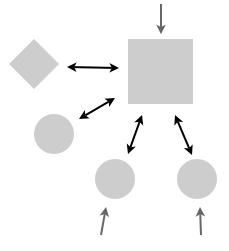
\includegraphics [scale=0.4] {img/other_model}
  \caption{\label{OthModel}
    {\small Existing models: cloud infrastructure with local
      caches. The circles represent high capacity devices, the diamond
      represents a mobile devices as smartphones or digital players,
      and the square represents the cloud infrastructure always
      available, in charge of resolving conflicting updates. Black
      arrows represent the connection and update propagation patterns
      while the grey arrows represent updates made to the user data.}}
\end{center}
\end{figure}

Unfortunately, we believe that the need for a central server has a few
drawbacks. The end-user has to trust the company providing the cloud
infrastructure for storing \emph{all} his data. Such models might
result into closed infratstructes tighted to the storage cloud
they rely on, where compatibility or migration between different
service providers might become difficult.

\subsection {pFS Personal Cloud Model}

In such
framework, users' mobile devices, even if considered as any other
devices by the system, become a very common relay for updates. Figure
\ref{PfsModel} shows a diagram of pFS model.

\begin{figure}[ht]
\begin{center}
  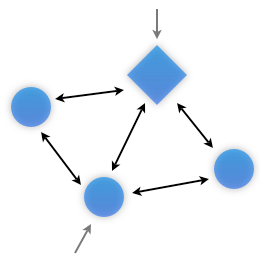
\includegraphics [scale=0.4] {img/pfs_model}
  \caption{\label{PfsModel} {\small pFS model: personal
      cloud. Updates are propagated between any couple of
      devices. The mobile devices appear as efficient relays 
      for updates.}}
\end{center}
\end{figure}






% Local Variables:
% tex-main-file: "main.ltx"
% tex-command: "make;:"
% tex-dvi-view-command: "make preview;:"
% End:
